\documentclass[11pt,a4paper]{article}
\usepackage[a4paper,hmargin=1in,vmargin=1in]{geometry}
\usepackage{pgfplots}
\pgfplotsset{compat=1.17}

\usepackage[czech]{babel}
\usepackage[utf8]{inputenc}
\usepackage[T1]{fontenc}

\usepackage{stddoc}
\usepackage{lipsum}
\usepackage{subcaption}

\newcommand{\plus}{{\texttt{+}}}
\renewcommand{\Re}{\operatorname{Re}}
\renewcommand{\Im}{\operatorname{Im}}
\newcommand{\fourier}[3]{\mathcal{F}_{#1}\!\left[#2\right]\!\left(#3\right)}
\newcommand{\ifourier}[3]{\mathcal{F}^{-1}_{#1}\!\left[#2\right]\!\left(#3\right)}


\begin{document}

\pagenumbering{arabic}

% Header
\begin{center}
    {\LARGE\textbf{Laboratorní úloha č. 5}}\\[3mm]
    \begin{minipage}{0.4\textwidth}
        \begin{flushleft}
            \textsc{\today}
        \end{flushleft}
    \end{minipage}
    ~
    \begin{minipage}{0.4\textwidth}
        \begin{flushright}
            \textsc{Martin Šimák}
        \end{flushright}
    \end{minipage}
    \noindent\rule{14.5cm}{0.4pt}
\end{center}

\paragraph*{Měření šumového čísla} Laboratorní úloha poskytuje seznámení se základními metodami měření šumového čísla pasivních i aktivních komponent. Úloha obsahuje měření jak zapomoci specializovaného měřiče, tak i pomocí spektrálního analyzátoru.

\subsection*{Úkoly měření}
\begin{enumerate}
    \item Měření šumového čísla spektrálního analyzátoru
    \item Měření šumového čísla pomocí Y-metody
    \item Měření šumového čísla pomocí HP 8970A
\end{enumerate}

\subsection*{Použité přístroje a komponenty}
\begin{itemize}
    \item Spektrální analyzátor R\&S FSP30 (9~kHz až 30~GHz)
    \item Měřič šumového čísla HP 8970A (10~MHz až 1,5~GHz)
    \item Šumivka HP 346B (do 18~GHz)
    \item Zesilovač Mini-Circuits ZX60-153LN-S\plus
    \item Stejnosměrný napájecí zdroj Gwinstek GPO-3303S 
    \item Propojovací BNC kabely
\end{itemize}

\subsection*{Měřené komponenty}
\begin{itemize}
    \item Nízkošumový zesilovač s tranzistorem BFP 840ESD
    \item Atenuátor Mini-Circuits s útlumem 8~dB
\end{itemize}

\subsection*{Popis měření}
\paragraph*{Nastavení spektrálního analyzátoru před měřením} Ještě před měření první úlohy je samozřejmě zapotřebí nastavit parametry spektrálního analyzátoru tak, aby měření probíhalo s co největší přesností. Toho dosáhneme nastavením hned několika parametrů:
\begin{itemize}
    \item vhodného rozsahu frekvencí (10 MHz až 5 GHz) s počtem bodů měření (sweep points) 501;
    \item šířky mezifrekvenčního filtru RBW na maximální hodnotu 10 MHz;%
    \footnote{Všechna měření na spektrálním analyzátoru budou spočívat v odečítání hodnot šumových výkonů, které následně budou porovnávány relativně vůči sobě. Měření je tedy na hodnotě RBW vlastně téměř nezávislé a toto nastavení volíme pouze z toho důvodu, že absolutní hodnota šumového výkonu je přímo úměrná RBW. V případě měření slabých deterministických signálů by ovšem muselo být RBW naopak co nejnižší.}
    \item hodnoty referenčního výkonu na -40 dBm, což zajistí nastavení maximálního zesílení na mezifrekvenčních blocích v analyzátoru před A/D převodníkem, a tedy využití celého dynamického rozsahu A/D převodníku;
    \item útlumu atenuátoru na vstupu analyzátoru na 0 dB;
    \item typ dekodéru na \emph{Detector Sample},
    aby zobrazovaný průběh skutečně ukazoval hladinu šumu na vstupu spektrálního analyzátoru.%
        \footnote{Ve spektrálním analyzátoru je jeden fyzický detektor z detekční diody a výkon v přijímaném pásmu heterodynního přijímače je určen pomocí navzorkovaného detekčního napětí na diodě. Nastavením typu detektoru na \emph{Detector Sample} v kategorii \emph{Trace} se na displeji zobrazují přímo detekované výkonu v pásmu RBW.}
\end{itemize}

% Task 1
\paragraph*{Měření šumového čísla spektrálního analyzátoru} První měření šumového čísla musíme provést na samotném spektrálním analyzátoru, neboť ten též k šumovému zkreslení nezanedbatelně přispívá. Měření provádíme metodou HOT/COLD s využitím šumivky, jíž zapnutím (\emph{Noise Src} na \emph{On}) se změní její ekvivalentní šumová teplota z $T_{\mathrm{COLD}} = T_0$ na $T_{\mathrm{HOT}} = T_0(ENR + 1)$, kde hodnota $ENR$ je na šumivce uvedena pro danou pracovní frekvenci a $T_0$ je nominální termodynamická teplota $290 \ \mathrm K$.

\begin{figure}[!ht]
    \centering
    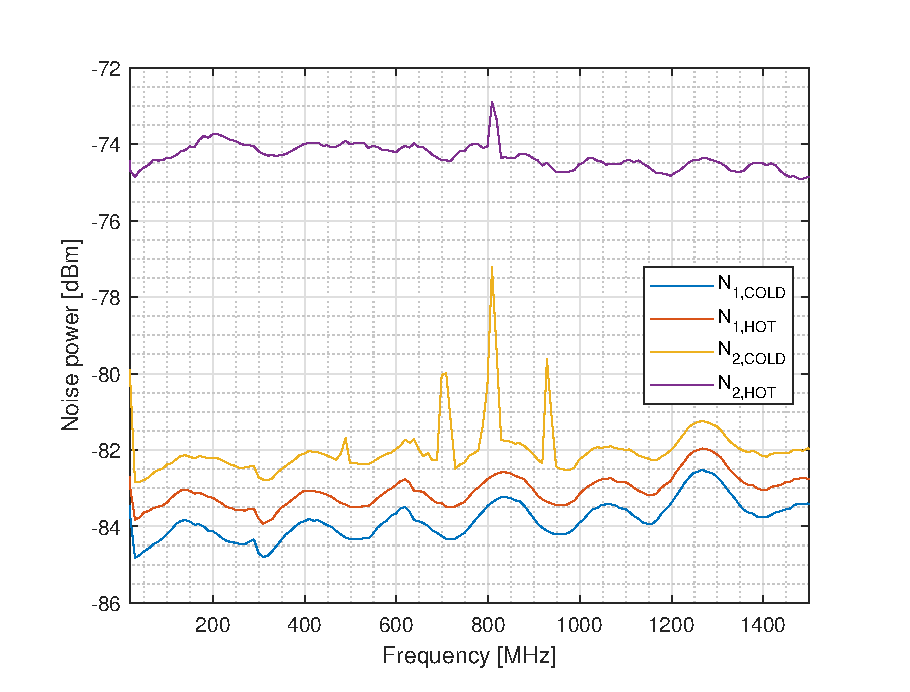
\includegraphics[width=.65\textwidth]{src/task1_powers.eps}
    \caption{Průběhy šumových výkonů}
    \label{fig:task1-powers}
\end{figure}
Zobrazované průběhy lze ze spektrálního analyzátoru exportovat do textového souboru (grafické znázornění na obrázku~\ref{fig:task1-powers}) a následně zpracovat pro získání šumového čísla. Tento jednoduchý postprocessing vychází přímo ze vztahů
\begin{align}
    Y_{\mathrm{SPA}} &= \frac{N_{\mathrm{HOT}}}{N_{\mathrm{COLD}}},
&
    F_{\mathrm{SPA}} &= \frac{ENR}{Y-1},
\end{align}
popřípadě lze dopočítat i ekvivalentní šumovou teplotu pomocí vztahu $T_e = T_0(F-1)$. V našem případě jsme takto postupovali pro dvě různé konfigurace: měření šumového čísla samotného spektrálního analyzátoru (1) a šumového čísla analyzátoru s předřazeným zesilovačem (2). Zpracované výsledky obou měření jsou graficky znázorněny na obrázcích~\ref{fig:task1-figures}~a~\ref{fig:task1-temperatures}.
\begin{figure}[!ht]
\centering
\begin{subfigure}{.45\textwidth}
    \centering
    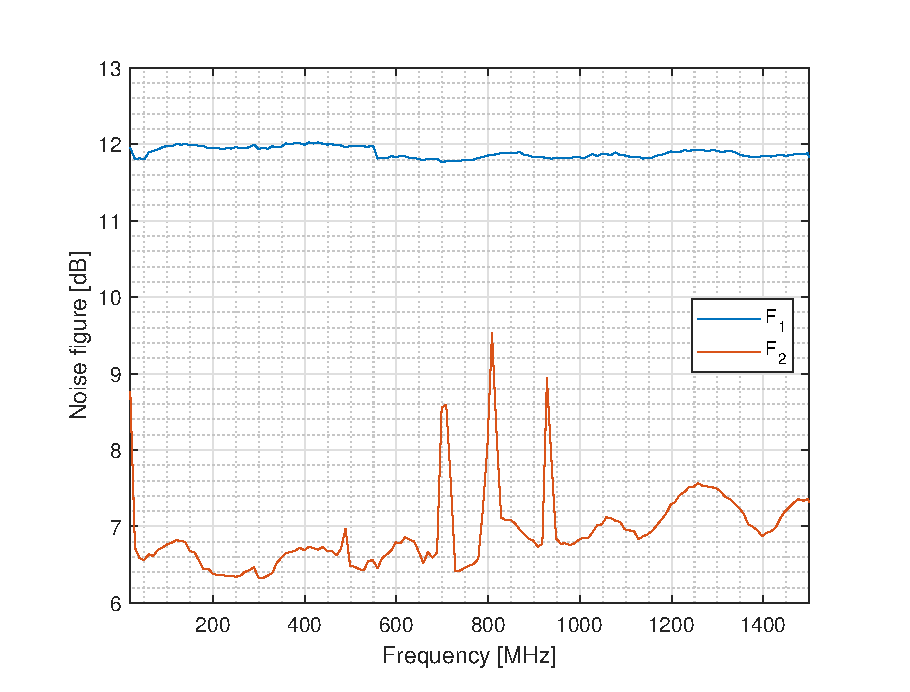
\includegraphics[width=\textwidth]{src/task1-figures.eps}
    \caption{Šumová čísla}
    \label{fig:task1-figures}
\end{subfigure}
\begin{subfigure}{.45\textwidth}
    \centering
    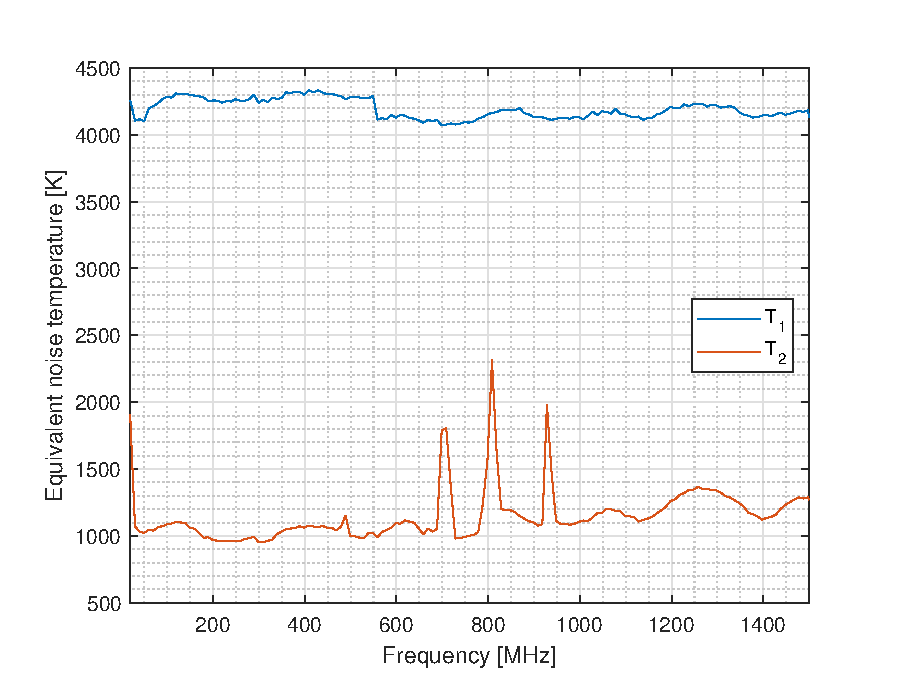
\includegraphics[width=\textwidth]{src/task1-temperatures.eps}
    \caption{Ekvivalentni šumové teploty}
    \label{fig:task1-temperatures}
\end{subfigure}
\caption{Grafické zpracování naměřených dat}
\end{figure}

\subparagraph*{Úkol} \emph{Zdůvodněte rozdíl mezi změřeným šumovým číslem samotného spektrálního analyzátoru a analyzátoru se zesilovačem.} Z obrázků~\ref{fig:task1-figures}~a~\ref{fig:task1-temperatures} jsou patrné hned dvě výrazné odlišnosti:
\begin{itemize}
    \item Průběhy se vzájemně liší zhruba o 5 dB, což je způsobeno tím, jak funguje kaskádování RF bloků z hlediska šumu, což je dáno Friisovým vztahem
    \begin{align}
        F_{\mathrm{AMT+SPA}} = F_{\mathrm{AMP}} + \frac{F_{\mathrm{SPA}}-1}{G_{\mathrm{AMP}}}.
    \end{align}
    To má za následek, že předřazení nízkošumového zesilovače před spektrální analyzátor značně snižuje šumové číslo měřící soustavy.
    \item Soustava s předřazeným zesilovačem má na specifických frekvencích značně vyšší hodnotu šumového čísla. To je způsobeno nedokonalým stínením předřazeného zesilovače, což má za následek průnik všudypřítomného rušivého signálu komunikačních služeb do obvodu zesilovače a tedy superpozici frekvenčně selektivního šumu na měřený signál.
\end{itemize}


% Task 2
\paragraph*{Měření šumového čísla Y-metodou pomocí spektrálního analyzátoru} Tato metoda je založena na Friisově vztahu pro výpočet šumového čísla kaskády RF bloků.
\begin{figure}[!ht]
    \centering
    \includegraphics[width=.65\textwidth]{src/task2-zapojeni.png}
    \caption{Zapojení úlohy měření šumového čísla Y-metodou}
    \label{fig:task2-zapojeni}
\end{figure}
Pro měření byla použita konfigurace na obrázku~\ref{fig:task2-zapojeni}, kde je zařazen zesilovač AMP před spektrálním analyzátorem pro zlešení přesnosti měření šumového čísla obvodu DUT. Zjištění šumového čísla kaskády AMP+SPA je tedy nutný kalibrační krok, jemuž bylo věnováno druhé měření v předchozí úloze. Pro uvedenou konfiguraci lze psát vztah
\begin{align}
    Y_{\mathrm{DUT+SPA}} = \frac{N_{\mathrm{HOT}}}{N_{\mathrm{COLD}}}.
\end{align}
Dosazením do vztahu pro výpočet šumového čísla dostáváme
\begin{align}
    \label{eq:F_DUT+SPA}
    F_{\mathrm{DUT+SPA}} = \frac{ENR}{Y_{\mathrm{DUT+SPA}}-1} = F_{\mathrm{DUT}} + \frac{F_{\mathrm{SPA}} - 1}{G_{\mathrm{DUT}}},
\end{align}
kde poslední rovnost plyne právě z Friisova vztahu. Ve výše uvedených vztazích přirozeně platí, že index SPA značí příslušnost veličiny spektrálnímu analyzátoru, index DUT měřenému zařízení a index SPA+DUT jejich kaskádě. Z rovnice~\ref{eq:F_DUT+SPA} tedy můžeme psát
\begin{align}
    F_{\mathrm{DUT}} = F_{\mathrm{DUT+SPA}} - \frac{F_{\mathrm{SPA}}-1}{G_{\mathrm{DUT}}},
\end{align}
kde $G_{\mathrm{DUT}}$ je zisk měřeného obvodu, který lze vyjádřit%
    \footnote{Dlužno podotknout, že zisk se v naprosté většině případů měří přímo pomocí skalárního či vektorového analyzátoru. My jsme uvedená data však měli připravené z předchozí úlohy, a tak bylo pohodlnější zisk získat touto nepřímou metodou.}
jako
\begin{align}
    G_{\mathrm{DUT}} = \frac{N_{2,\mathrm{HOT}} - N_{2,\mathrm{COLD}}}{N_{1,\mathrm{HOT}} - N_{1,\mathrm{COLD}}},
\end{align}
přičemž veličiny s indexem 2 odpovídají měřením šumových výkonů obvodu s DUT (šumové výkony na obrázku~\ref{fig:task2-powers}) a měření s indexem 1 obvodu bez DUT (šumové výkony $N_2$ na obrázku~\ref{fig:task1-powers}). Frekvenční průběhy samotných zisků jsou vyneseny na obrázku~\ref{fig:task2-gains}.
\begin{figure}[!ht]
    \centering
    \begin{subfigure}{.45\textwidth}
        \centering
        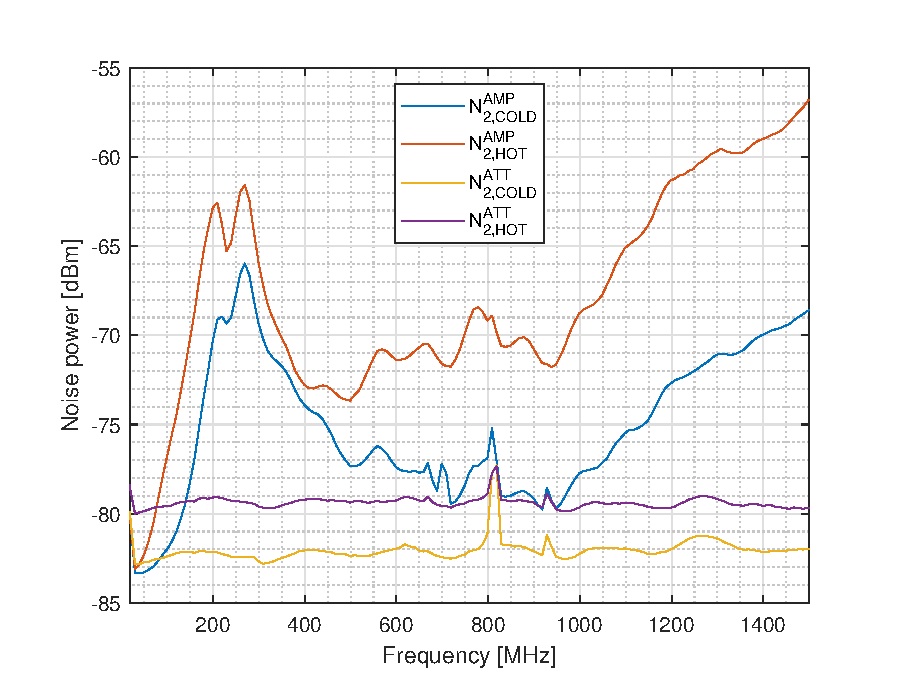
\includegraphics[width=\textwidth]{src/task2-powers.eps}
        \caption{Šumové výkony za stavů HOT a COLD}
        \label{fig:task2-powers}
    \end{subfigure}
    \begin{subfigure}{.45\textwidth}
        \centering
        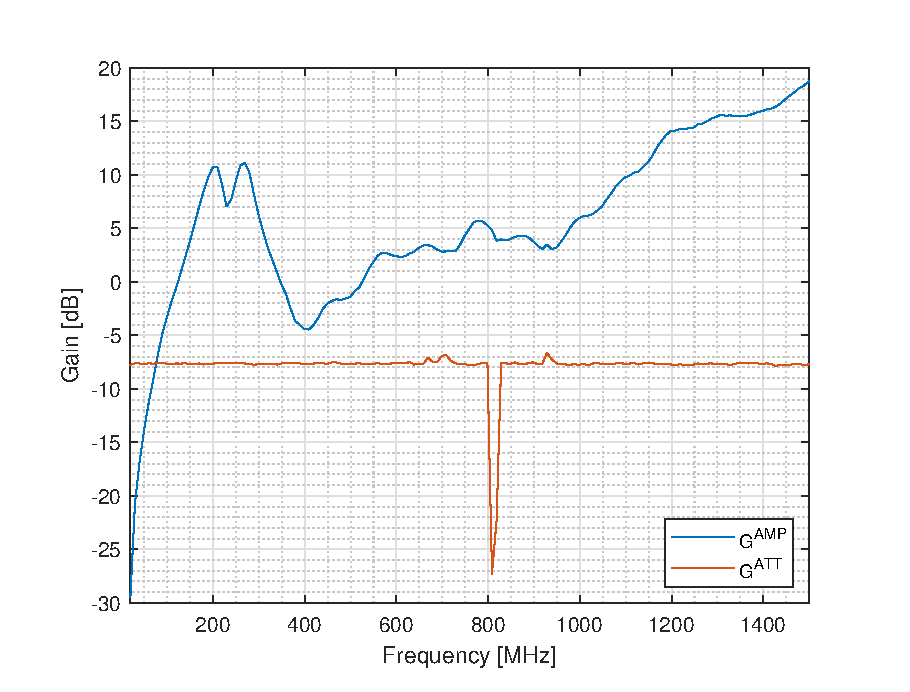
\includegraphics[width=\textwidth]{src/task2-gains.eps}
        \caption{Zisky}
        \label{fig:task2-gains}
    \end{subfigure}
    \caption{Změřená data pro zesilovač a atenuátor}
\end{figure}

Výsledky zpracování dat (výpočet šumových čísel a ekvivalentních šumových teplot) jsou k nahlédnutí na obrázcích~\ref{fig:task2-figures}~a~\ref{fig:task2-temperatures}.
\begin{figure}[!ht]
    \centering
    \begin{subfigure}{.45\textwidth}
        \centering
        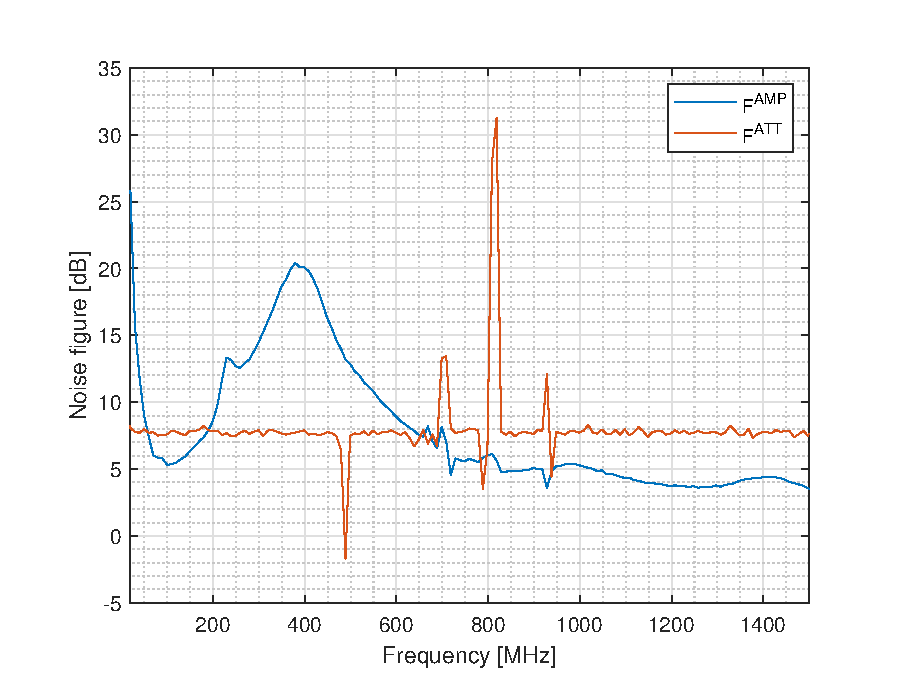
\includegraphics[width=\textwidth]{src/task2-figures.eps}
        \caption{Šumová čísla}
        \label{fig:task2-figures}
    \end{subfigure}
    \begin{subfigure}{.45\textwidth}
        \centering
        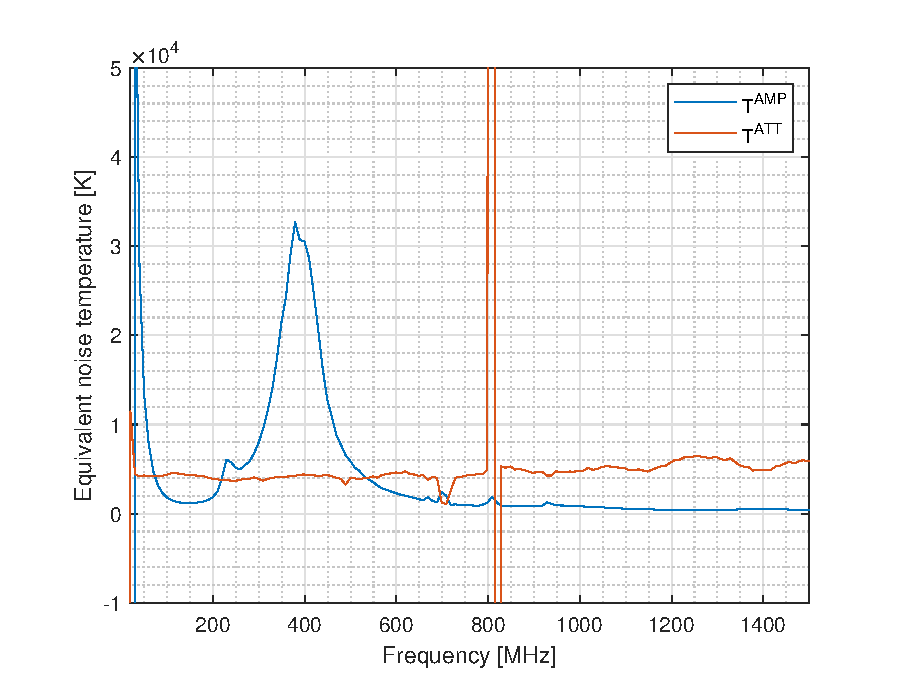
\includegraphics[width=\textwidth]{src/task2-temperatures.eps}
        \caption{Ekvivalentní šumové teploty}
        \label{fig:task2-temperatures}
    \end{subfigure}
    \caption{Grafické zpracování naměřených dat}
\end{figure}

% Task 3
\paragraph*{Měření šumového čísla pomocí měřiče HP 8970A} V rámci této úlohy měříme šumové číslo a zisk DUT přímo pomocí specializovaného měřiče šumového čísla. Nejprve je potřeba měřič zkalibrovat, čehož lze dosáhnout připojením šumivky a zmáčknutím tlačítka \emph{Calibrate}. Na přístroji proběhne rutina spočívající ve změření šumového čísla měřícího přístroje v defaultním frekvenčním rozsahu 30 MHz až 1,5 GHz po kroku 20 MHz. Pomocí tlačítek v sekci
\emph{Smoothing} se dá měnit počet průměrovaných změřených hodnot na každé frekvenci. Měření i kalibrace ovšem potom probíhá pomaleji, nicméně změřené hodnoty jsou stabilnější. Defaultně průměrování neprobíhá.

Výsledky měření šumového čísla a zisku DUT (zesilovač a atenuátor) připojeného mezi šumivku a měřič jsou zaneseny v tabulkách~\ref{table:task3-amp}~a~\ref{table:task3-att}.
\begin{table}[!ht]
\begin{center}
\begin{tabular}{| l || c | c | c | c | c | c | c | c |}
    \hline
    $f \ [\mathrm{MHz}]$ & 100 & 300 & 500 & 700 & 900 & 1100 & 1300 & 1500 \\
    \hline\hline
    $G_{\mathrm{DUT}} \ [\mathrm{dB}]$ & -2,4 & 7,5 & -0,5 & 4,2 & 4,8 & 9,5 & 15,4 & 18,4 \\
    \hline
    $F_{\mathrm{DUT}} \ [\mathrm{dB}]$ & 6,4 & 14,0 & 12,8 & 6,7 & 5,0 & 4,1 & 3,5 & 3,3 \\
    \hline
\end{tabular}
\caption{Tabulka naměřených hodnot pro zesilovač}
\label{table:task3-amp}
\end{center}
\end{table}

\begin{table}[!ht]
\begin{center}
\begin{tabular}{| l || c | c | c | c | c | c | c | c |}
    \hline
    $f \ [\mathrm{MHz}]$ & 100 & 300 & 500 & 700 & 900 & 1100 & 1300 & 1500 \\
    \hline\hline
    $G_{\mathrm{DUT}} \ [\mathrm{dB}]$ & -7,6 & -7,6 & -7,6 & -7,6 & -7,6 & -7,6 & -7,6 & -7,6 \\
    \hline
    $F_{\mathrm{DUT}} \ [\mathrm{dB}]$ & 7,6 & 7,7 & 7,8 & 7,7 & 7,8 & 7,7 & 7,8 & 7,6 \\
    \hline
\end{tabular}
\caption{Tabulka naměřených hodnot pro atenuátor}
\label{table:task3-att}
\end{center}
\end{table}

\subparagraph*{Úkol} \emph{Porovnejte hodnoty s šumovými čísly a zisky změřených pomocí Y-metody v předchozí úloze.} Hodnoty se příliš neliší až na nízké frekvence, kde se dá předpokládat příčina v nepřesnosti měření spektrálního analyzátoru.

\subsection*{Závěr}
V rámci laboratorní úlohy jsme se seznámili s měřením šumového čísla pasivních i aktivních mikrovlnných obvodů. Měření jsme prováděli jak pomocí specializovaného měřice, tak i poněkud manuálnější metodou využívající pouze spektrálního analyzátoru. Měření proběhlo bez větších problémů a výsledky odpovídají znalostem nabitým během teoretických přednášek o měření šumových parametrů.


\end{document}
